\documentclass[a4paper,12pt]{article}
\usepackage{graphicx}       %LaTeX package to import graphics

\usepackage[T1]{fontenc}
\usepackage[italian]{babel}

\usepackage{subcaption}

\usepackage{hyphenat}
\usepackage{array}
\usepackage{booktabs}       % Per linee orizzontali migliori
\usepackage{caption}        % Per personalizzare le didascalie<
\usepackage{multirow}       % Per combinare celle nelle colonne
\usepackage{hyperref}

\usepackage{bm} 

\usepackage{amsmath}        % Per migliorare l'aspetto delle formule

\usepackage{todonotes}      % mettere le note dentro il documento

\usepackage{siunitx}        % Per formattare le unità di misura
\usepackage{gensymb}        % Simboli come °
\usepackage{xfrac}          % per fare le frazioni inclinate

\usepackage{pdfpages}

\usepackage{import}
\usepackage{frontespizio}

\usepackage{placeins}       %per non far andare le immagini al di fuori delle sezioni utilizzare il comando: \FloatBarrier non far superare le immagini quel punto

\usepackage{adjustbox}      % per dimensionare le immagini in modo automatico


\addto\extrasitalian{\renewcommand{\figureautorefname}{figura}}
\addto\extrasitalian{\renewcommand{\AMSautorefname}{equazione}}
\addto\extrasitalian{\renewcommand{\tableautorefname}{tabella}}

\begin{document}


\includepdf{./frontespizio/frontespizio.pdf}

\section*{Progettazione Circuito Digitale}

Dato un numero $X$ compreso tra $0$ e $15$, rappresentabile tramite $4$ bit, l’obiettivo è stato quello di realizzare un circuito digitale in grado di fornire in uscita $Q = 1$ se e solo se $X \geq 10$. Poiché sono necessarie $16$ combinazioni ($2^4$), l’idea è stata quella di utilizzare un componente \textit{dip switch} a $4$ interruttori. I $4$ bit in ingresso all’integrato 4093, composto da 4 porte NAND, sono forniti dal \textit{dip switch} stesso collegato come \autoref{fig:mappa-karnaugh}. Chiudendo l’interruttore, il bit passa da 0 a 1 mentre aprendolo passa da 1 a 0. In uscita all’integrato 4093 è stata collegata una resistenza di circa $2\, \mathrm{k} \ohm $ con in serie un LED per verificare il corretto funzionamento del circuito: il LED si accende quando $X \geq 10$ e rimane spento quando $X < 10$. La tensione di alimentazione del circuito è pari a $5\,\mathrm{V}$.

\begin{align*}
	b_2 \cdot b_3 + b_3 \cdot b_1 \qquad \Rightarrow \qquad \overline{\overline{b_2 \cdot b_3} \cdot \overline{b_3 \cdot b_1}}\\
\end{align*}

\begin{figure}[h]
	\centering
	
\includegraphics[width=0.8\linewidth]{immagini/circuito-digitale/circuito.png}
	\caption{Schematico circuito implementato.}
	\label{fig:schematico-circuito}
\end{figure}


\begin{table}[h]
	\centering
	\setlength{\tabcolsep}{10pt}
	\begin{tabular}{ c || c|c|c|c | c}
		X  & $b_3$ & $b_2$ & $b_1$ & $b_0$ & \bf{Q} \\
		\midrule
		0  & 0     & 0     & 0     & 0     & 0 \\
		1  & 0     & 0     & 0     & 1     & 0 \\
		2  & 0     & 0     & 1     & 0     & 0 \\
		3  & 0     & 0     & 1     & 1     & 0 \\
		4  & 0     & 1     & 0     & 0     & 0 \\
		5  & 0     & 1     & 0     & 1     & 0 \\
		6  & 0     & 1     & 1     & 0     & 0 \\
		7  & 0     & 1     & 1     & 1     & 0 \\
		8  & 1     & 0     & 0     & 0     & 0 \\
		9  & 1     & 0     & 0     & 1     & 0 \\
		10 & 1     & 0     & 1     & 0     & 1 \\
		11 & 1     & 0     & 1     & 1     & 1 \\
		12 & 1     & 1     & 0     & 0     & 1 \\
		13 & 1     & 1     & 0     & 1     & 1 \\
		14 & 1     & 1     & 1     & 0     & 1 \\
		15 & 1     & 1     & 1     & 1     & 1 \\
	\end{tabular}
	\caption{Tabella della verità.}
	\label{tab:tabella-verita}
\end{table}

\begin{figure}[h]
	\centering
	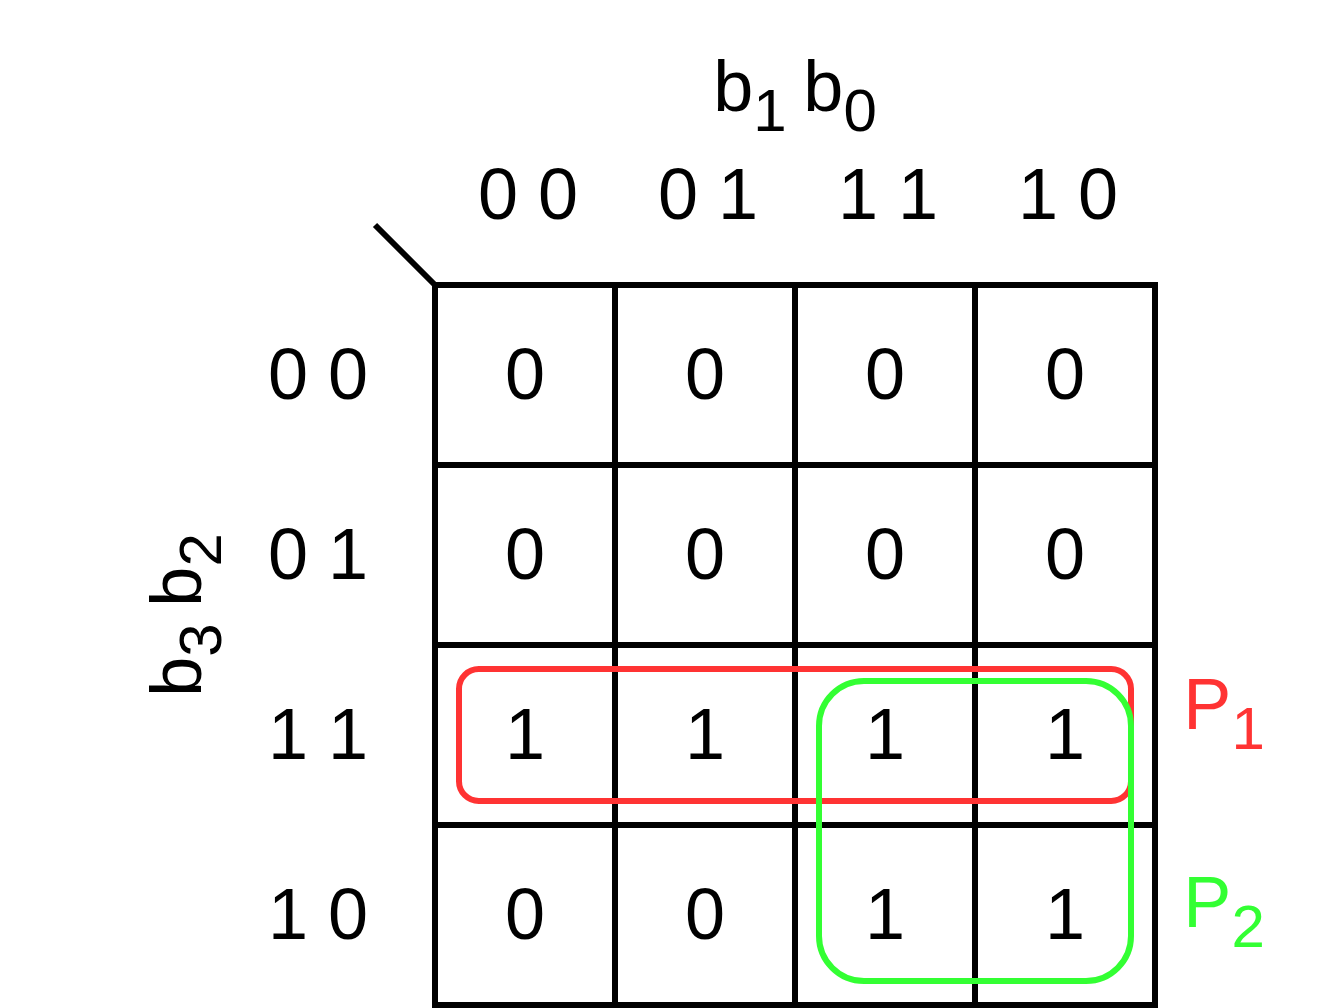
\includegraphics[width=0.65\linewidth]{immagini/circuito-digitale/mappa_di_karnaugh.png}
	\caption{Mappa di Karnaugh.}
	\label{fig:mappa-karnaugh}
\end{figure}


\FloatBarrier

\section{Timer 555}

Il timer 555 è un circuito integrato molto diffuso grazie alla sua versatilità. 
Internamente è composto da:

\begin{itemize}
	\item un partitore resistivo che crea due soglie di riferimento, una a $\dfrac{1}{3} V_{cc}$  e l'altra a $\dfrac{2}{3} V_{cc}$;
	\item due comparatori che confrontano la tensione sul condensatore con queste due soglie;
	\item un latch set-reset che determina lo stato in uscita seguito poi da una porta NOT che determina l'uscita vera e propria;
	\item un MOSFET di scarica assimilabile a un interruttore. 
\end{itemize}

Questi blocchi permettono di realizzare diverse configurazioni operative:
\begin{itemize}
	\item Monostabile: genera un impulso di durata predefinita in presenza di un impulso di trigger.
	\item Bistabile: viene utilizzato come flip-flop set-reset mantenendo il segnale di uscita finché non arriva un segnale di set/reset.
	\item Astabile: produce una forma d'onda periodica senza bisogno di segnali esterni. 
\end{itemize}

% Da mettere comunque? Oppure da cancellare dato che è scritto simile nel primo item del primo itemize?
%Nel circuito la $V_{cc}$ viene ripartita equamente con 3 resistenze uguali. In questo modo compaiono 2 comparatori: uno a soglia %$\sfrac{2}{3}$ (sopra) e uno a soglia $\sfrac{1}{3}$ (sotto).


\subsection{Monostabile}
Questa configurazione viene utilizzata per effettuare switch debouncing. 
Gli interruttori, generalmente, sono soggetti a un rimbalzo meccanico quando premuti e, per tale motivo, si hanno impulsi spuri. La configurazione monostabile genera un impulso di durata fissata da R e C, non influenzato dal rimbalzo.
Per acquisire correttamente l'impulso è stata utilizzata la modalità “single” dell’oscilloscopio, impostando il trigger a $\mathrm{V_{DD}/2} = 5\,\mathrm{V}$ sul fronte di discesa del segnale.
Per ottenere una durata dell’impulso di circa 2 secondi, il circuito è stato dimensionato con i valori riportati a \autoref{tab:valori-monostabile}.
Inoltre è stato aggiunto un LED finale, collegato al resto del circuito tramite una resistenza da $2.1\,\mathrm{k}\ohm$, per verificare il corretto funzionamento della presente configurazione.


\begin{align*}
	t = 1.1 \cdot R_1 \cdot C_1
\end{align*}

\begin{table}[h]
	\centering
	\setlength{\tabcolsep}{20pt}
	\begin{tabular}{c c}
		\toprule
		\textbf{Grandezza} & \textbf{Valore}         \\
		\midrule
		$C$                & $19.5\,\mu\mathrm{F}$   \\
		$R_1$              & $101.5\,\mathrm{k}\ohm$ \\
		$R_2$              & $11.8\,\mathrm{k}\ohm$  \\
		\bottomrule
	\end{tabular}
	\caption{Valori utilizzati nel circuito: Monostabile.}
	\label{tab:valori-monostabile}
\end{table}

\subsection{Astabile}
In questa configurazione il periodo e il duty cycle dipendono dal circuito RC esterno.
Nel nostro caso quest'ultimo è uguale a $\frac{T_1}{T}$ cioè pari a $\frac{R_A+R_B}{R_A + 2 R_B}$. 
Di conseguenza la carica del condensatore dipende da $R_A+R_B$ mentre la scarica dal solo $R_B$.
Dimensionando il circuito per ottenere una frequenza di $1\,\mathrm{kHz}$, sono stati scelti $R_A= 11.8\,\mathrm{k}\ohm$, $R_B=4.7\,\mathrm{k}\ohm$ e $C = 70\,\mathrm{nF}$.
È stato poi verificato che il periodo teorico,
\[
T = T_1 + T_2 = \ln 2 \cdot (R_A + 2 R_B) C,
\]
coincidesse con quello misurato.

\end{document}